%%%%%%%%%%%%%%%%%%%%%%%%%%%%%%%%%%%%%%%%%%%%%%%%%%%%%%%%%%%%%%%%%%%%%%%%
%
% First comes an example EPS file -- just ignore it and
% proceed on the \documentclass line
% your LaTeX will extract the file if required
\begin{filecontents*}{example.eps}
%!PS-Adobe-3.0 EPSF-3.0
%%BoundingBox: 19 19 221 221
%%CreationDate: Mon Sep 29 1997
%%Creator: programmed by hand (JK)
%%EndComments
gsave
newpath
  20 20 moveto
  20 220 lineto
  220 220 lineto
  220 20 lineto
closepath
2 setlinewidth
gsave
  .4 setgray fill
grestore
stroke
grestore
\end{filecontents*}
%
\RequirePackage{fix-cm}
%
%\documentclass{svjour3}                     % onecolumn (standard format)
%\documentclass[smallcondensed]{svjour3}     % onecolumn (ditto)
\documentclass[smallextended]{svjour3}       % onecolumn (second format)
%\documentclass[twocolumn]{svjour3}          % twocolumn
%
\smartqed  % flush right qed marks, e.g. at end of proof
%
% \usepackage{mathptmx}      % use Times fonts if available on your TeX system
%
% insert here the call for the packages your document requires
%\usepackage{latexsym}
% etc.
%
\usepackage{graphicx}
\usepackage[round]{natbib}
\usepackage{amssymb,amsmath}
%
% please place your own definitions here and don't use \def but
\newcommand{\mnras}{MNRAS}
\newcommand{\nat}{Nature}
\newcommand{\aap}{A\&A}
\newcommand{\apj}{ApJ}
\newcommand{\apjl}{ApJL}
\newcommand{\physrep}{Phys.Rep.}
\newcommand{\prd}{Phys.Rev.D}
\newcommand{\araa}{ARA\&A}
\newcommand{\Ddt}{D_{\Delta{\rm t}}}
\newcommand{\Dd}{D_{\rm d}}
\newcommand{\Ds}{D_{\rm s}}
\newcommand{\Dds}{D_{\rm ds}}
\newcommand{\zd}{z_{\rm d}}
\newcommand{\zs}{z_{\rm s}}
\newcommand{\cospars}{\boldsymbol{\Omega}}
\newcommand{\x}{\boldsymbol{\theta}}
\newcommand{\y}{\boldsymbol{\beta}}
\newcommand{\grad}{\boldsymbol{\nabla}}
\newcommand{\deflectionangle}{\boldsymbol{\alpha}}
%
% Insert the name of "your journal" with
% \journalname{myjournal}
%
%%%%%%%%%%%%%%%%%%%%%%%%%%%%%%%%%%%%%%%%%%%%%%%%%%%%%%%%%%%%%%%%%%%%%%%%

\begin{document}

\title{Time delay cosmography%\thanks{Grants or other notes
%about the article that should go on the front page should be
%placed here. General acknowledgments should be placed at the end of the article.}
}
%\subtitle{Time delay cosmography}

\titlerunning{Time delay lens cosmography}        % if too long for running head

\author{Tommaso Treu         \and
        Philip J. Marshall %etc.
}

%\authorrunning{Treu \& Marshall} % if too long for running head

\institute{Tommaso~Treu \at
Department of Physics and Astronomy, \\
University of California,\\
Los Angeles, CA 90095, USA\\
\email{tt@astro.ucla.edu}           %  \\
%             \emph{Present address:} of F. Author  %  if needed
           \and
Philip~J.~Marshall \at
Kavli Institute for Particle Astrophysics and Cosmology, \\
P.O. Box 20450, MS29, \\
Stanford, CA 94309, USA \\
}

\date{Received: date / Accepted: date}
% The correct dates will be entered by the editor

\maketitle

%%%%%%%%%%%%%%%%%%%%%%%%%%%%%%%%%%%%%%%%%%%%%%%%%%%%%%%%%%%%%%%%%%%%%%%%

\begin{abstract}

Gravitational time delays, observed in strong lens systems where the
variable background source is multiply-imaged by a  massive galaxy in
the foreground, provide direct measurements of cosmological distance
that are very complementary to other cosmographic probes. The success of
the technique depends on the availability and size of a suitable sample
of lensed quasars or supernovae, precise measurements of the time
delays, accurate modeling of the lens mass distributions, and our
ability to characterize the density environment along the line of sight
to the source. We review the progress made during the last 15 years,
during which the first competitive cosmological inferences with time
delays were made, and look ahead to the potential of significantly
larger lens samples in the near future.

% TT: Mention blindness? PJM: I'm not sure it belongs here - it's not unique to time delays, and abstracts of reviews shoudl be especially short...

\keywords{First keyword \and Second keyword \and More}
% \PACS{PACS code1 \and PACS code2 \and more}
% \subclass{MSC code1 \and MSC code2 \and more}

\end{abstract}

%%%%%%%%%%%%%%%%%%%%%%%%%%%%%%%%%%%%%%%%%%%%%%%%%%%%%%%%%%%%%%%%%%%%%%%%

\section{Introduction [TT]}
\label{sec:intro}

The measurement of cosmic distances is central to our understanding of
cosmography, i.e. the description of the geometry and kinematics of
the universe. The discovery of the period luminosity relation for
Cepheids led to the realization that the universe is much bigger than
the Milky Way and that it is currently expanding. Relative distance
measurements based on supernova Ia light curves were the turning point
in the discovery of the acceleration of the universe
\citep{Riess:1998p21184,Per++99}.

In the two decades since the discovery of the acceleration of the
universe, distance measurements have improved steadily. For example,
the Hubble constant has now been measured to 2.4\% precision
\citep{Rie++16} while the distance to the last scattering surface of
the cosmic microwave backgrond is now known to approximately 0.5\%
precision \citep[depending on the assumed cosmological
model]{WMAP9,Pla15}. This precision is more than sufficient for all
purposes related to our understanding of phenomena occurring within
the universe, like galaxy evolution.

In spite of all this progress, the most fundamental question still
remains unanswered. What is causing the acceleration? Is this {\it
dark energy} something akin to Einstein's cosmological constant or is
it a dynamical component? Answering this question from an empirical
standpoint will require further improvements in the precision of
distance measurements \citep{Suy++12,Wei++13,Kim++15,Rie++16}.  In
practice, measuring the dark energy equation of state requires an
accurate model of the scale parameter of the universe as a function of
time, particularly when dark energy is dynamically most relevant,
i.e. below $z\sim1$.

%\begin{figure}[!t]
%\begin{center}
%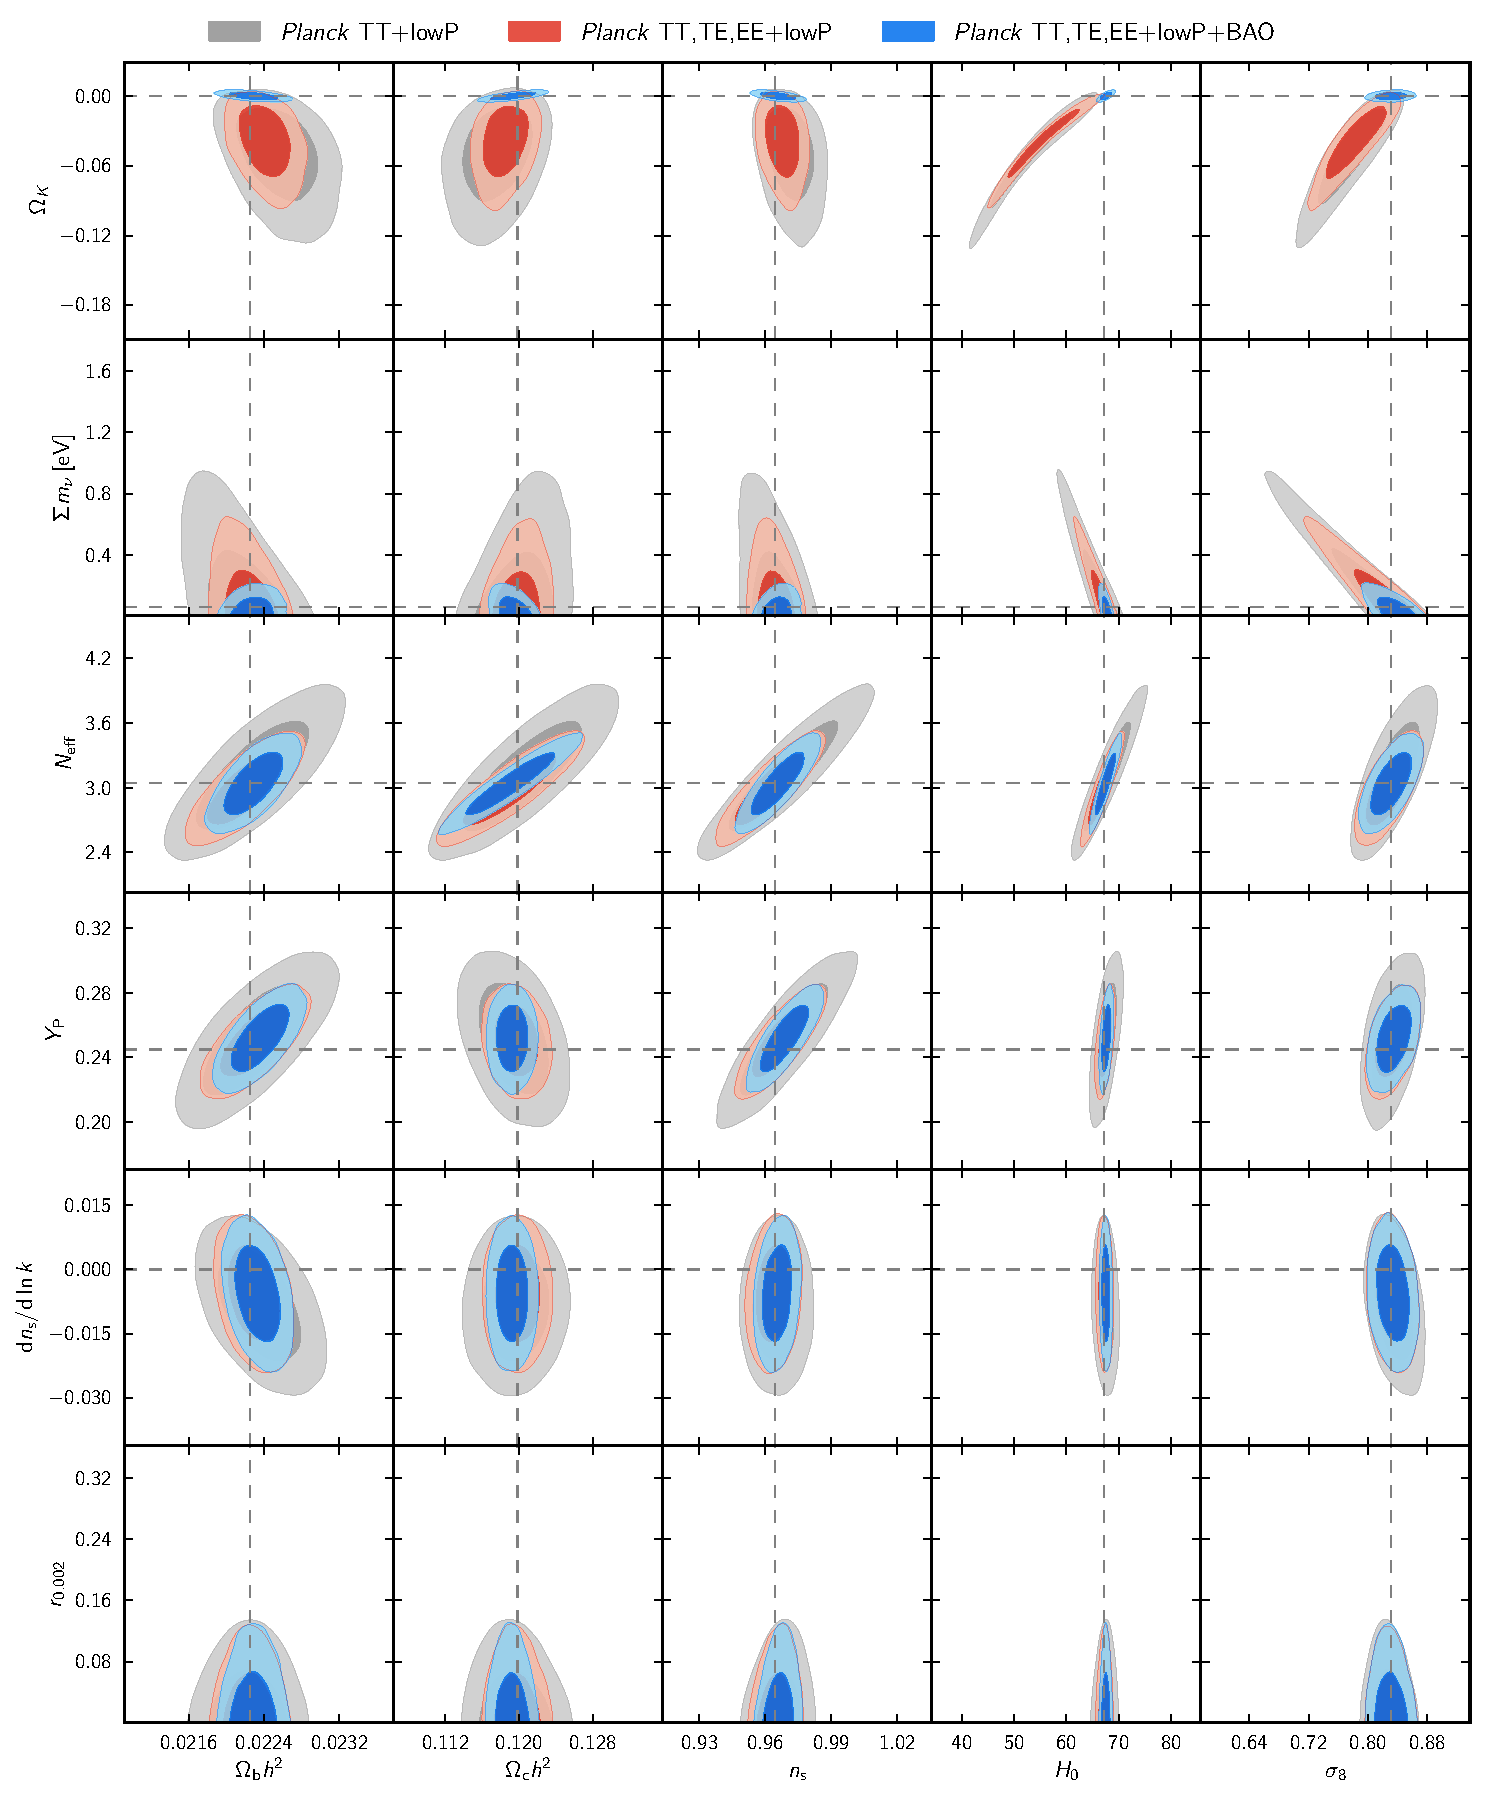
\includegraphics[width=0.5\textwidth]{figures/grid_1paramext.pdf}
%\caption{The figure, taken from \cite{Pla15}, shows the confidence
%intervals obtained for 1-parameter extension of the basic $\Lambda$CDM
%model obtained using Plank measurements themselves, and in combination
%with baryonic acoustic oscillations. Note that the interpretation of
%CMB data long is strongly degenerate, even in these simple
%models. Lower redshift distance measurements, in case from BAO, break
%the degeneracies. See the original paper \cite{Pla15} for details
%about the figure and input parameters.}
%\label{fig:CMB}
%\end{center}
%\end{figure}

Cosmic microwave background anisotropies primarily provide a
measurement of the angular distance to the last scattering surface,
obtain by comparing the angular scale of the acoustic peaks with the
baryonic acoustic oscillation scale. Therefore, the constraints set by
CMB anisotropy data on dark energy parametere are highly degenerate in
a generic cosmological model
\citep[e.g.,][]{Pla15}. Breaking the degeneracy requires strong
assumptions about the universe (e.g., flatness or dark energy being
the cosmological constant), or lower redshift distance
measurements. Many dedicated experiments are currently under way or
being planned with this goal in mind.

%A summary of distance
%measurements with approximate precision and redshift range is given in
%Figure~\ref{fig:comparedist}.
%[Include distance ladder, CMB, BAO, cosmic clocks, fgas]

%\begin{figure}[!t]
%\begin{center}
%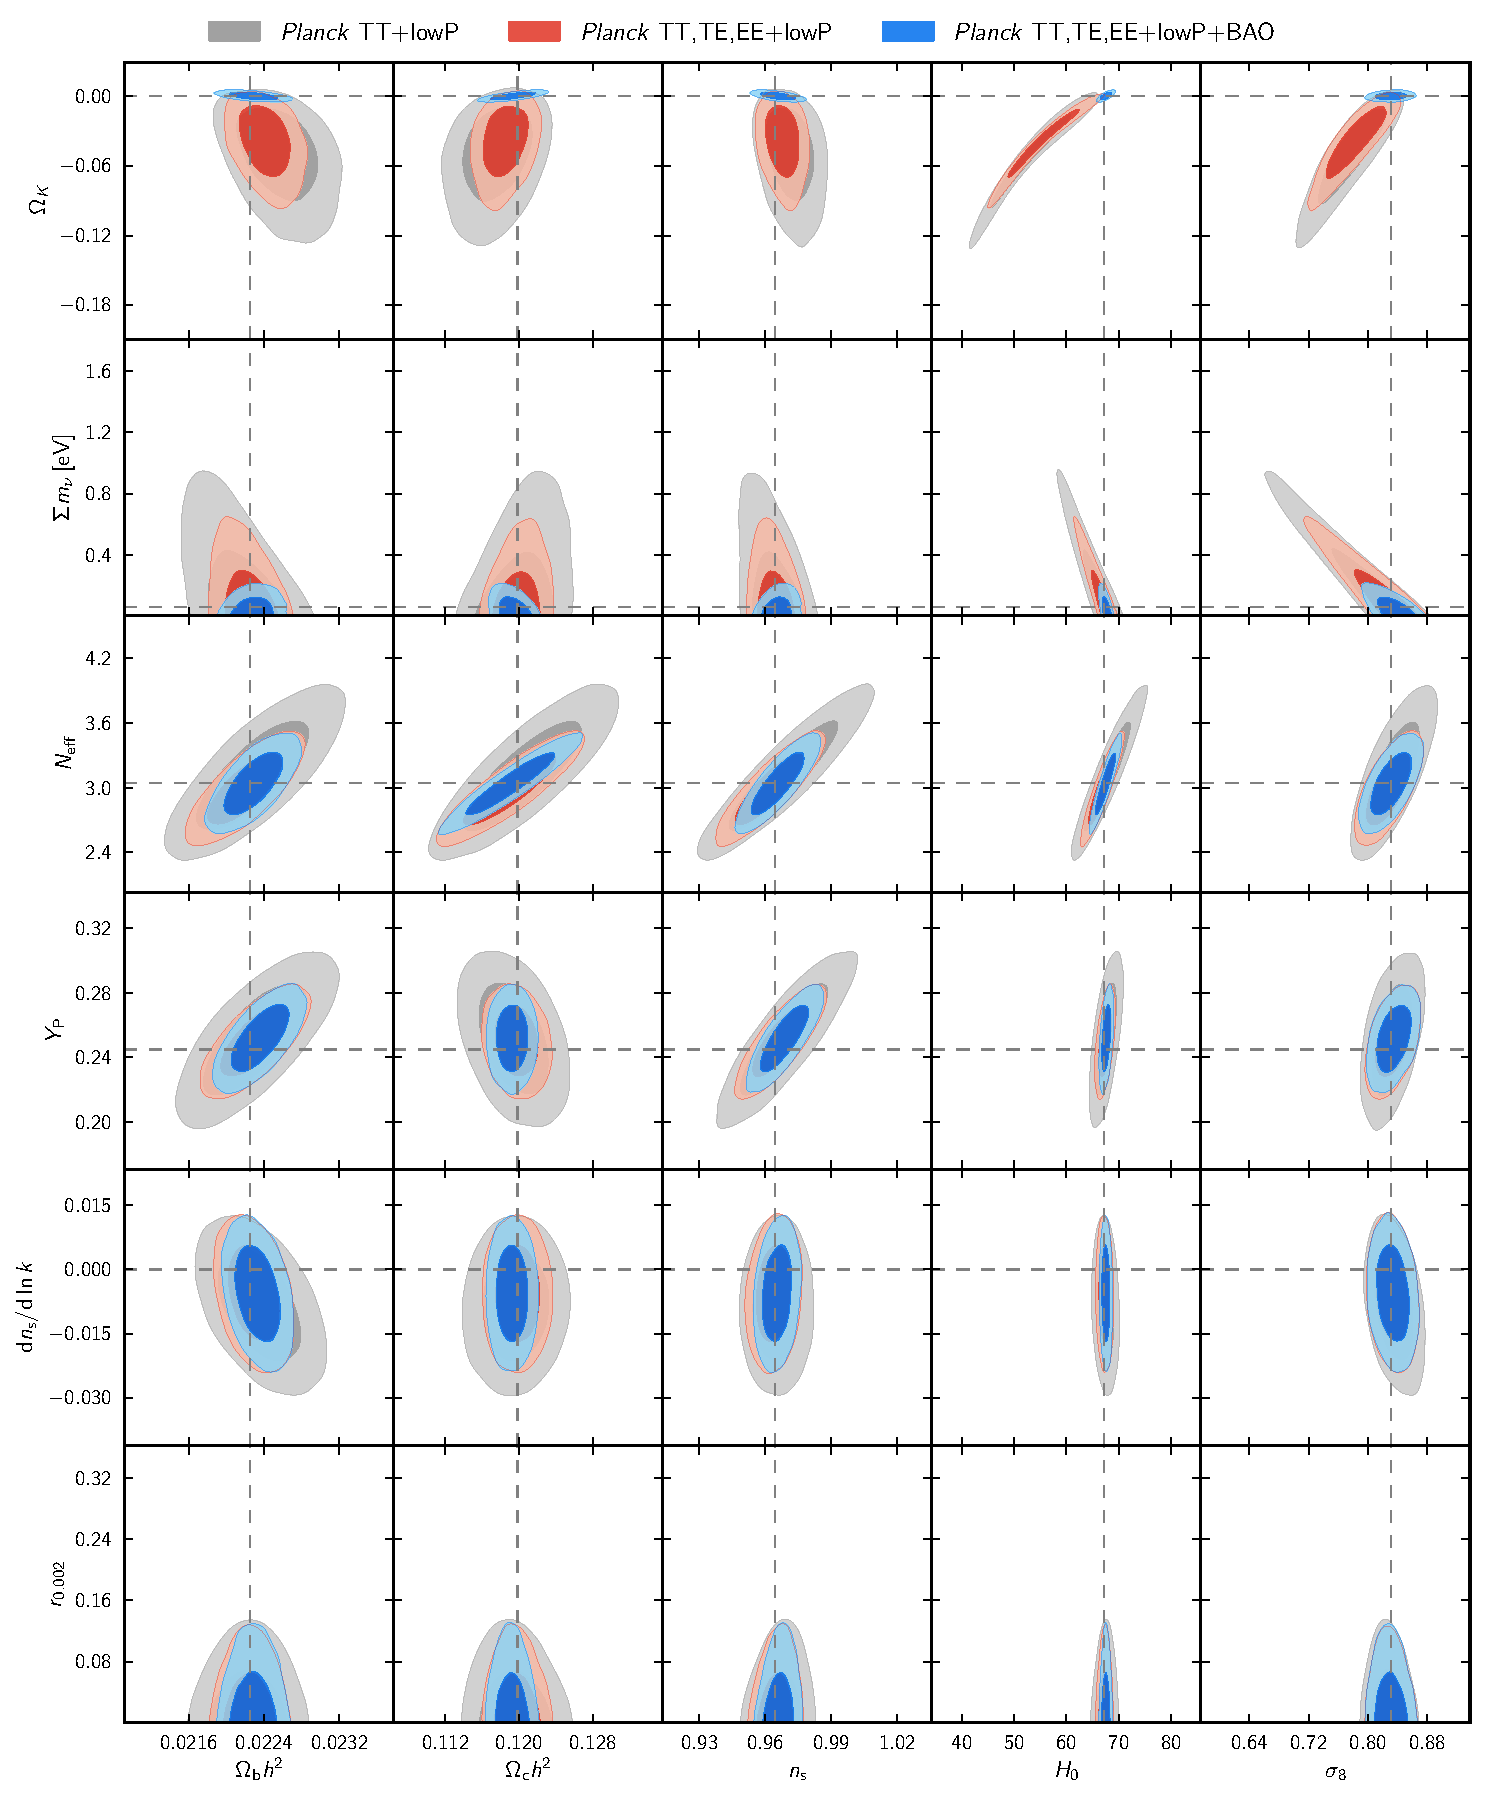
\includegraphics[width=0.5\textwidth]{figures/grid_1paramext.pdf}
%\caption{Summary of current distance measurements}
%\label{fig:comparedist}
%\end{center}
%\end{figure}

Precision, however, is not sufficient by itself. In addition to
controlling the known statistical uncertainties ({\it precision}),
modern day experiments need to control systematic errors ({\it
accuracy}) in order to fullfill their potential, including the
infamous unknown unknowns. The most direct way to demonstrate accuracy
is to compare independent measurements that have comparable precision. An
interesting, currently topical, and relevant case is that of the 3$-\sigma$ tension
between the local distance ladder determination of H$_0$
\citep{Rie++16} and that inferred by the Plank satellite assuming a
flat $\Lambda$CDM model \citep{Pla15}. The tension could be due to an
unknown source of systematic errors in either or both of the two measurements, or
it could be indicative of new physics, for example an effective number of
relativistic species greater than three. Independent measurements with
comparable precision are the best way to make progress.
% For example,
% the WMAP9 measurement \citep{Cal++13} is significantly less in tension
% with the cosmic distance ladder data than the Planck one.
While independent measurements of the same phenomenon, or reanalysis of the
same data \citep{Efs14,SFH15}, are certainly useful and necessary,
completely independent datasets based on different physical phenomena
provide qualitatively new information.

Ideally, the comparison between independent measurements should be
carried out blindly, so as to minimize experimenter bias. Two mutually
blind measurements agreeing that the equation of state parameter $w$
is not $-1$ would be a very convincing demonstration that the dark
energy is not the cosmological constant. Conversely, the significant
disagreement of two blind and independent measurements, could be the
first sign of new physics.

In this review we focus on strong lensing gravitational time delays as
a tool for cosmography. As we shall see, this probe provides a direct
and elegant way to measure absolute distances out to cosmological
redshift. When the line of sight to a distant source of light is
suitably well aligned with an intervening massive system, multiple
images appear to the observer. The arrival time of the images depends
on the interplay of the geometric and gravitational delays specific to
the configuration. If the emission from the source is variable in
time, the difference in arrival time is measurable, and can be
interpreted via a so-called ``time delay distance'' $\Ddt$.
In the simplest case, this distance is just a multiplicative combination
of the three angular diameter distances between the observer, deflector and
source. $\Ddt$ is
inversely proportional to the Hubble Constant $H_0$, and more
weakly dependent on other cosmological parameters. As several authors
have pointed out \citep{Hu05,Lin11,Suy++12,Wei++13}, achieving
sub-percent precision and accuracy on the measurement of the Hubble
constant will be a powerful addition to Stage III and IV dark energy
experiments. The independence of time delays from other traditional
probes of cosmology, makes them very valuable for precise and accurate
cosmology. For example, time delays yield an {\it absolute}
measurement of distance without relying on Cepheids or any other local
rung of the distance ladder, and because the relevant quantities are
angular diameter distances rather then luminosity distances, the
approach is insensitive to dust or
other photometric errors.

This review is organized as follows. In Section~\ref{sec:intro} we
summarize the history of time delay cosmography up until the turn of
the millennium, in order to give a sense of the early challenges and
how they were overcome. In Section~\ref{sec:theory}, we review the
theoretical foundations of the method, in terms of the gravitational
optics version of Fermat's principle. In Section~\ref{sec:measurement}
we describe in some detail the elements of a modern time delay
distance measurement, emphasizing recent advances and remaining
challenges. In Section~\ref{sec:cosmo} we elucidate the connection
between time delay distance measurements and cosmological parameters,
discussing complementarity with other cosmological
probes. Section~\ref{sec:outlook} critically examines the future of
the method, discussing prospects for increasing the precision, testing
for accuracy, and synergy with other future probes of dark energy. A
brief summary is given in Section~\ref{sec:summary}.

Owing to space limitations, we could only present a selection of all
the beautiful work that has been published on this topic in the past
decades. We refer the readers to recent
\citep{Bar10,Ell10,Tre10,TMC12,Jackson:2013p30763,Jac15,T+E15}
and not-so-recent \citep{B+N92,CSS02,K+S04,Fal05,SKW06}
excellent reviews and textbooks \citep{SEF92} for additional
information and historical context.


%%%%%%%%%%%%%%%%%%%%%%%%%%%%%%%%%%%%%%%%%%%%%%%%%%%%%%%%%%%%%%%%%%%%%%%%

\section{A brief history of time delay cosmography [TT]}
\label{sec:history}

\citet{Ref64} first suggested that strong lens time delays could be
used to measure absolute, cosmological distances, and
therefore the Hubble Constant to leading order. Unfortunately, no
strong lensing systems were known at that time, and therefore his
intuition remained purely theoretical for over a decade.

The prospects of using time delays for cosmography suddenly brightened
in the late seventies, with the discovery of the first strongly lensed
quasar \citep{WCW79}. Even though they were not the strongly lensed
supernovae that Refsdal had had in mind, quasar fluxes are sufficiently
variable \citep{Van82} that people were able to start to put Refsdal's
idea in practice \citep{Van89}.
The first multiply imaged supernova was discovered in 2014,
fifty years afer Refsdal's initial suggestion \citep{Kel++15}, lensed
by a foreground cluster of galaxies. The time delays are being
measured at the time of writing
\citep{Rod++16,Kel++16}; however, it is unclear at the moment whether the
cluster potential can be constrained with sufficient accuracy to
yield interesting cosmological information \citep{Tre++16}. In general,
we expect the more straightforwardly-modeled, more numerous
galaxy-scale time delay lenses to be the most useful systems for
cosmography, with supernovae competing for attention with quasars \citep{O+M10}.
In this review, we will restrict our case to the to date much more common and
better understood case of variable active galactic nuclei (AGN) being lensed by
foreground elliptical galaxies.

Discovery and monitoring of lensed quasars continued in the eighties and
nineties, powered by heroic efforts. By the end of the millennium the
number of known strongly lensed systems was in double digits
\citep{CSS02}, and the first truly robust time delays were measured
\citep{Kun++97,Sch++97}.
The industrial detection of multiply imaged AGN finally took off at the
beginning of the current millennium, with the improvement of panoramic
search technology in dedicated or existing surveys
\citep{Bro++03,Oguri:2006p5865,Agn++15}.

The initial period of time delay cosmography was marred by controversies over
systematic errors.  The measurement of time delays was particularly
controversial during the nineties as the quality of the early data
allowed for multiple estimated values \citep{PRH92}, owing to the combined
effects of gaps in the data, and microlensing noise in the optical
light curves. This problem was solved definitively at the turn of the
millennium, with the beginning of modern monitoring campaigns,
characterized by high cadence, high precision, and long duration, both
at optical and radio wavelengths
\citep{Fas++99,Fas++02,Bur++02,Eig++05}, as illustrated in
Figure~\ref{fig:oldvsmoderndt}. We discuss
modern monitoring campaigns in more detail in Section~\ref{ssec:timedelay}.

%%%%%%%%%%%%%%%%%%%%%%%%%%%%%%%%%%%%%%
\begin{figure*}
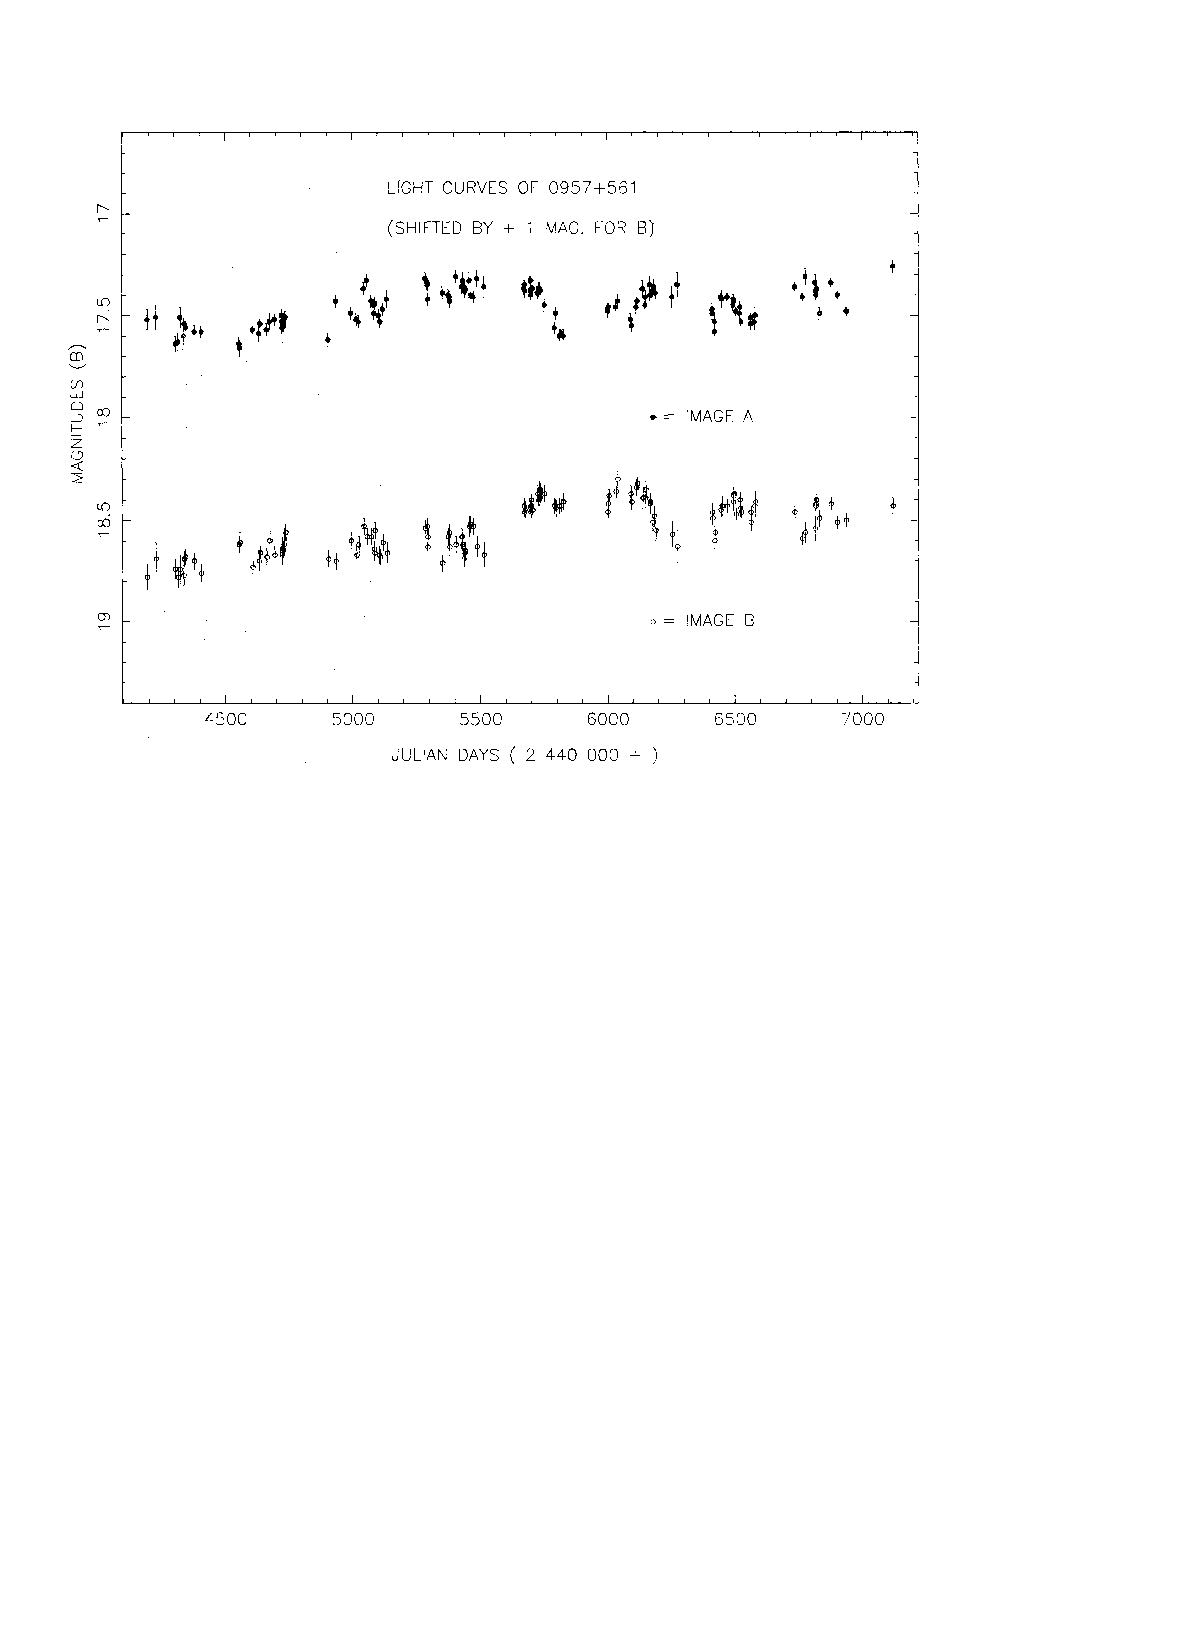
\includegraphics[width=0.48\textwidth]{figures/Vanderriest89_fig5.pdf}
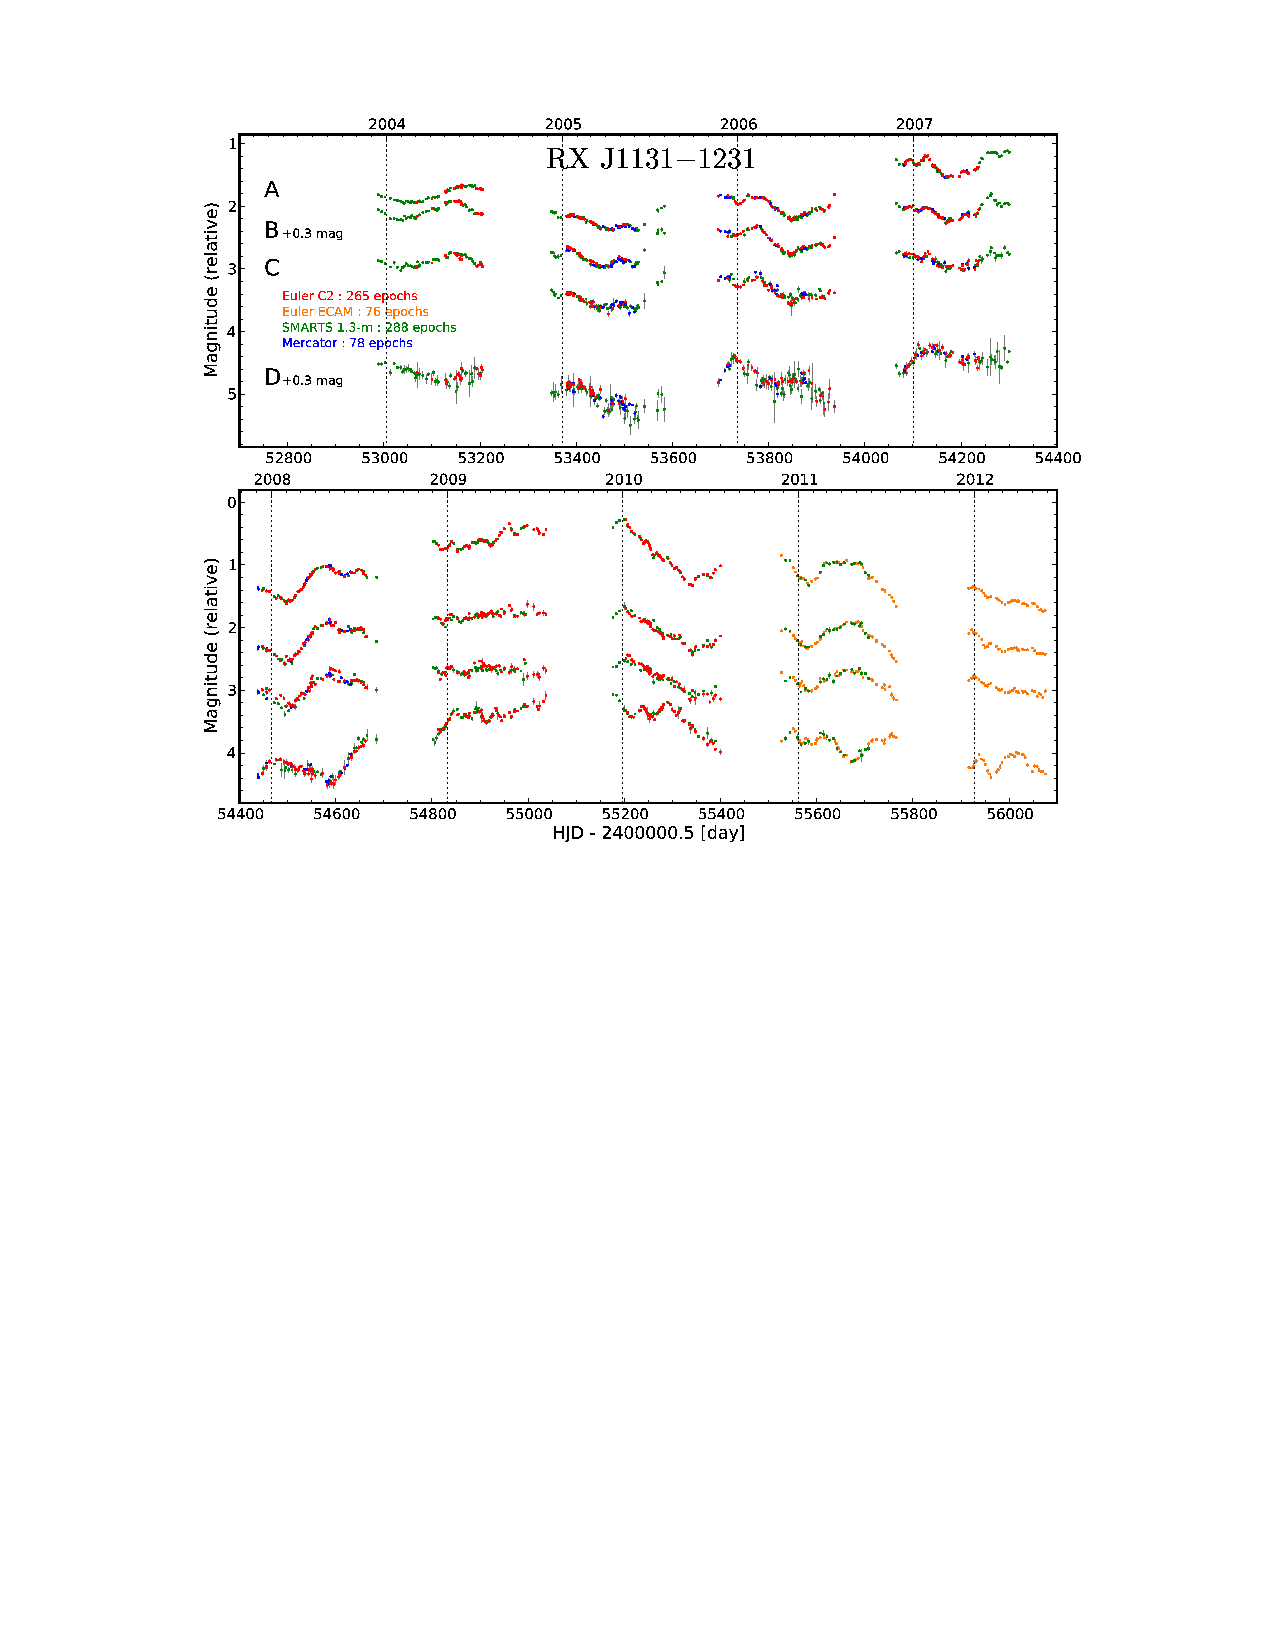
\includegraphics[width=0.48\textwidth]{figures/Tewes13-fig4.pdf}
\caption{Comparison between one of the early light curves \citep[left
panel, from][]{Van89}, and a modern light curve from COSMOGRAIL
\citep[right panel, from][]{Tew++13}. Note the improved photometric
precision, cadence, and duration of the light curves, allowing for
unambiguous determination of the time-delay to within 1-2\% precision.}
\label{fig:oldvsmoderndt}
\end{figure*}
%%%%%%%%%%%%%%%%%%%%%%%%%%%%%%%%%%%%%%

Finally, when robust time delays started to become available, the
focus of the controversy shifted to the modeling of the gravitational
potential of the lens. Typically, in the mid nineties, the only
constraints available to modelers were the quasar image positions and
to lesser extent flux ratios (limited by microlensing, variability and
differential extinction). Thus, the best one could do was to assume
some simple form for the lens mass distribution, such as a singular isothermal
sphere,
% thus breaking the mass sheet degeneracy,
and to neglect the
effects of structure along the line of sight. Given these necessary
but oversimplistic assumptions, random errors grossly underestimated
the total uncertainty, leading to measurements that were apparently
significantly inconsistent
between groups, or with those from other techniques
\citep{K+S04}. Since then, two methods have been pursued in order to
% break degeneracies in more flexible modeling of the lensing data and
obtain realistic estimates of the uncertainties. One consists of using
large samples of systems with relatively weak priors
\citep{Ogu07b}. The other method consists of obtaining high quality data for
each lens system, including detailed imaging of the quasar host galaxy
\citep{Keeton:2000p241,WBB04,Suy++06}, or non-lensing data like the deflector
stellar velocity dispersion \citep{T+K02b} and the properties of
galaxies along the line of sight \citep{K+Z04,Suy++10}. We discuss
these approaches in Section~\ref{ssec:lensmodel}. The astounding
improvement in data quality over the past two decades is illustrated
in Figure~\ref{fig:oldvsmodernimage}.

%%%%%%%%%%%%%%%%%%%%%%%%%%%%%%%%%%%%%%
\begin{figure*}
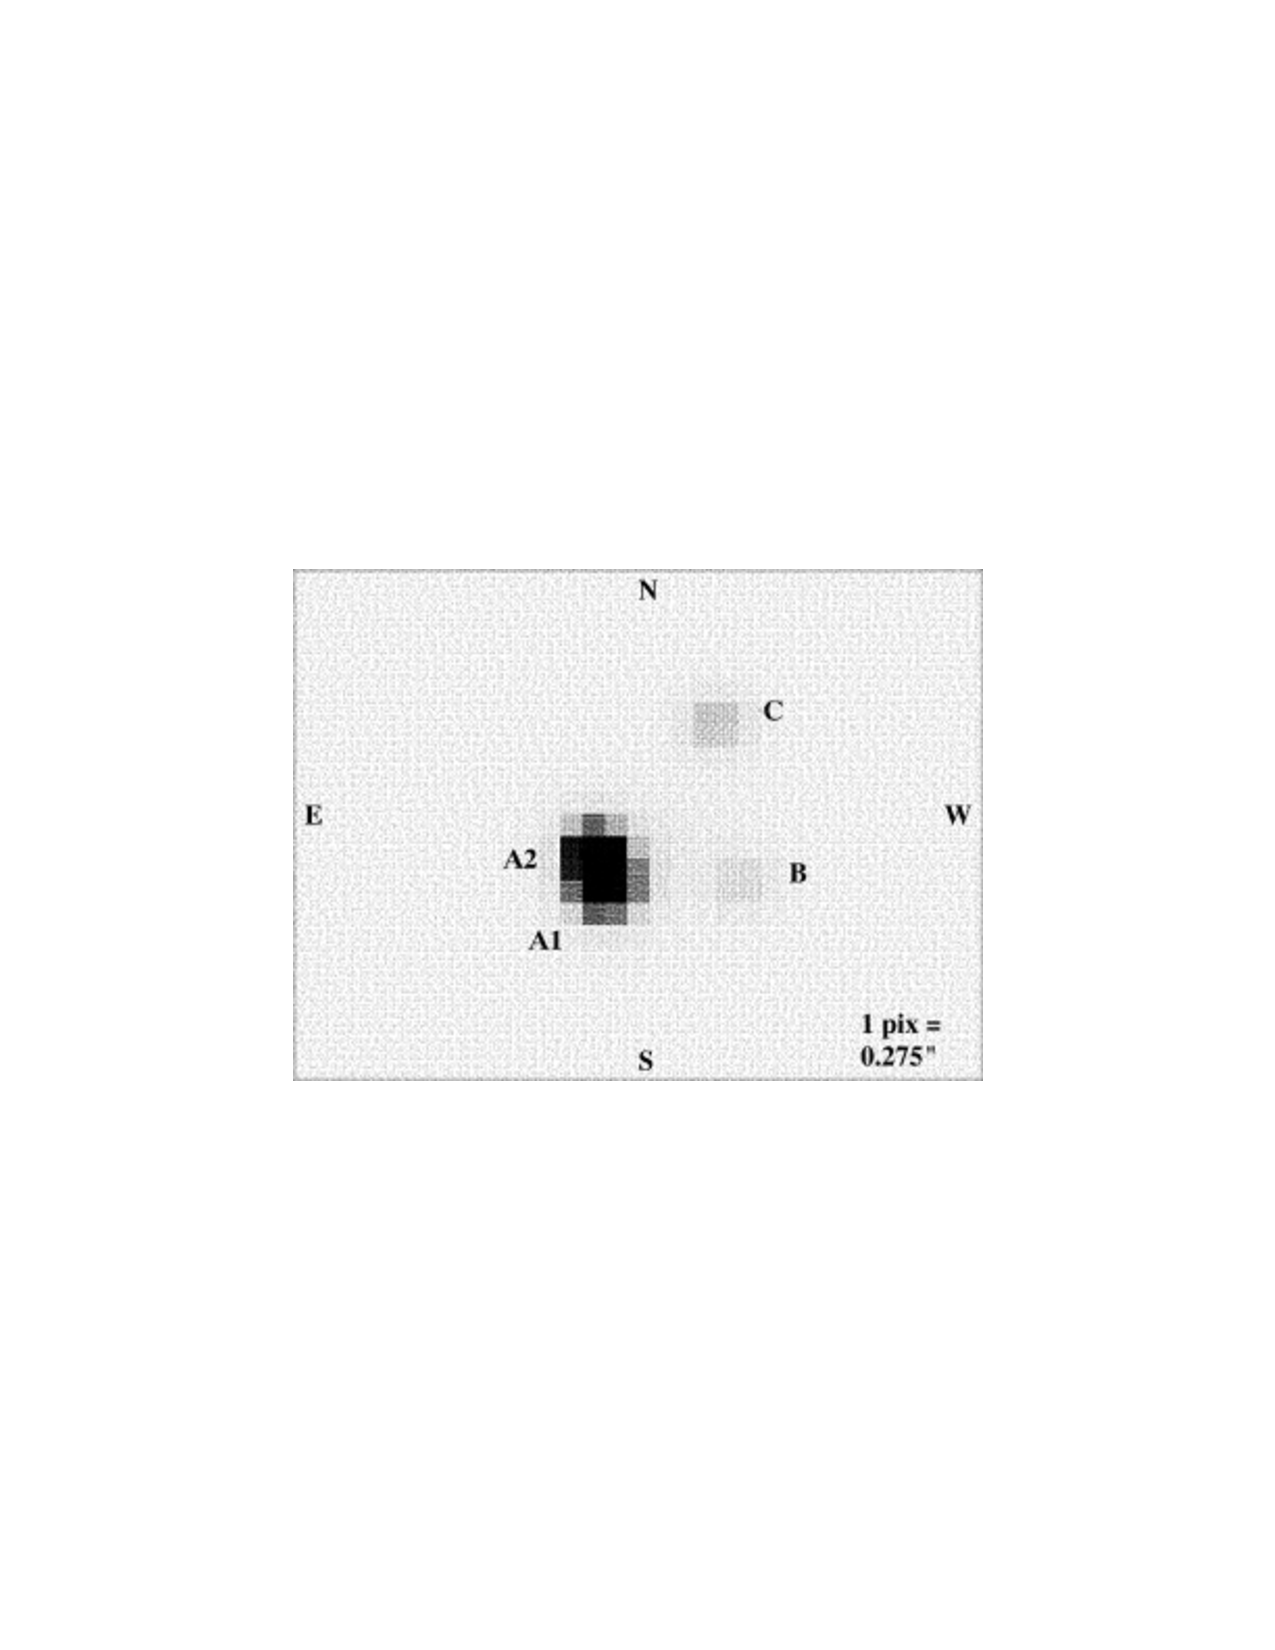
\includegraphics[height=3.5cm]{figures/Schechter97_fg1.pdf}
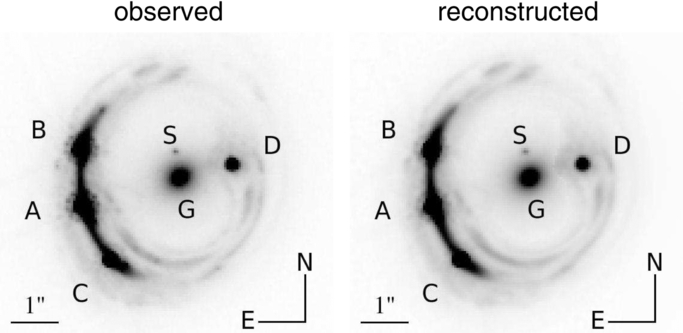
\includegraphics[height=3.5cm]{figures/Suyu14_fig1.jpg}
\caption{Comparison between imaging data available in the nineties
\citep[eft panel, from][]{Sch++97} and in the most recent studies
\citep[middle and right panels, from][]{Suy++14}). With modern data the
structure of the quasar host galaxy can be modeled in great detail,
providing thousands of constraints on the deflection angle, and thus on
the derivatives of the gravitational potential.}
\label{fig:oldvsmodernimage}
\end{figure*}
%%%%%%%%%%%%%%%%%%%%%%%%%%%%%%%%%%%%%%

Ultimately, the controversies over systematic errors were essential to
spur the community to overcome the difficulties and find ways to
address them. This is a natural and probably inevitable part of the
scientific process. However, the bitterness of some of those
controversies during the ninenties and early naughties still resonates
today: unfortunately, some of the scientists that followed the field
with excitement at that time are still under the impression that
strong lensing time delays are inherently inaccurate and imprecise. As
we have briefly described here, and we will show in detail in the
next sections, in the last twenty years the field has moved forward
considerably implementing many solutions to the lessons learned the
hard way.


%%%%%%%%%%%%%%%%%%%%%%%%%%%%%%%%%%%%%%%%%%%%%%%%%%%%%%%%%%%%%%%%%%%%%%%%

\section{Theoretical background [PJM]}
\label{sec:theory}


In this section we provide a brief summary of the theory of
gravitational lens time delays. We have distilled much of the content
of this section from the excellent exposition of Schneider and
Kochanek \citep{SKW06}, as well as the various key papers we cite.

% Lensing, Fermat's principle and potential. Time delay surface.

Fermat's Principle of Least Time holds for the propagation of light rays
through curved spacetime. The light travel time through an isolated, thin
gravitational lens is given by
%
\begin{align}
    \tau(\x) &= \frac{\Ddt}{c} \cdot \Phi(\x,\y), \\
    \text{where\;\;} \Phi(\x) &= \frac{1}{2}\left(\x - \y\right)^2 - \psi(\x).
\end{align}
%
Here, $\x$ denotes the light source's apparent position on the sky, and
$\y$ is the position of the unlensed source. The difference between the
observable position~$\x$ and the unobservable position~$\y$ is the
scaled deflection angle~$\deflectionangle({\x})$, which is typically
$\sim1$~arcsecond in a galaxy-scale strong gravitational lens system.
$\psi(\x)$ is the scaled gravitational potential of the lensing object,
projected onto the lens plane. Both $\deflectionangle(\x)$ and $\psi(\x)$ can be
predicted given a model for the mass distribution of the lens.

Images form at the extrema of the light travel time, where $\grad
\tau(\x) = \grad \Phi(\x) = 0$ \citep{Schneider1985}. For this reason,
$\Phi(\x)$ is known as the ``Fermat potential.'' This quantity can also
be thought of as the spatially-varying refractive index of the lens. The
arrival time itself is not observable, but differences in arrival time
between multiple images are. In the above approximation, the  ``time delay'' $\Delta \tau_{\rm AB}$
between image A and
image B can be predicted via
%
\begin{equation}
    \Delta \tau_{\rm AB} = \frac{\Ddt}{c} \Delta \Phi_{\rm AB} \label{eq:timedelay}
\end{equation}
%
where $\Delta \Phi_{\rm AB}$ is the Fermat potential difference between the
two image positions.
Figures~\ref{fig:timedelaycartoon} and~\ref{fig:delays} illustrate the origin of the
time delay between the images in a gravitational lens system. The small
magnitude of the fractional time delay (typically $\Delta\tau \sim 10$~days out of
$\Ddt/c \sim 10^{12}$ days light travel time)
is commensurate with the square of the
deflection angle (typically $|\deflectionangle|\sim1$~arcsecond, or $\sim 5\times10^{-6}$
radians).

\begin{figure*}[!t]
\centering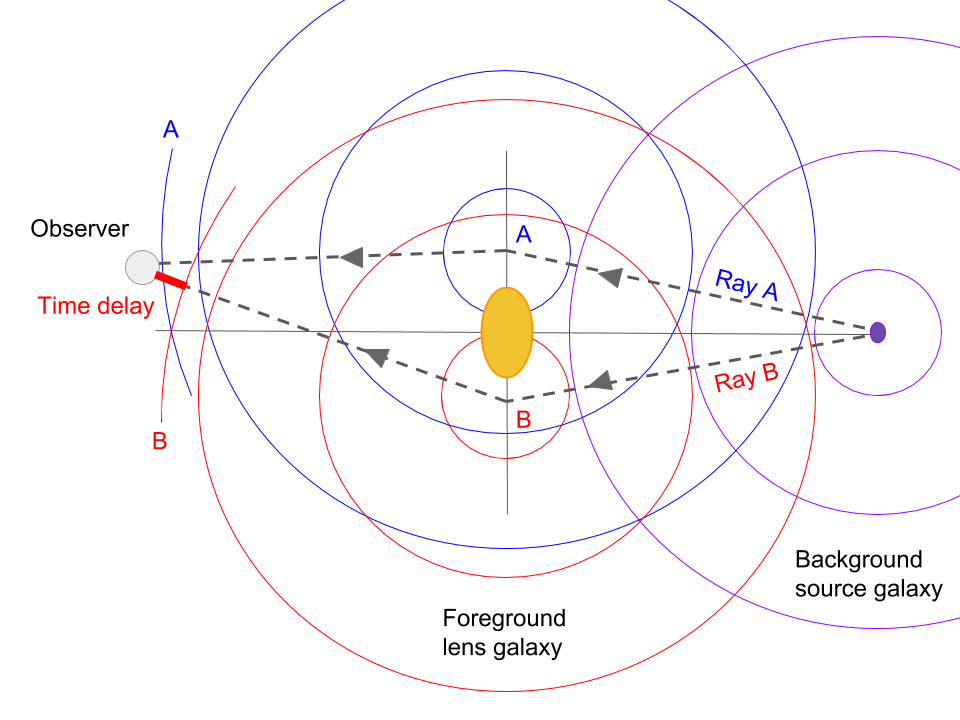
\includegraphics[width=0.96\textwidth]{figures/wavefront-schematic.png}
\caption{Schematic diagram
illustrating the origin of the gometric component of the time delay.}
\label{fig:timedelaycartoon}
\end{figure*}

\begin{figure*}[!ht]
\centering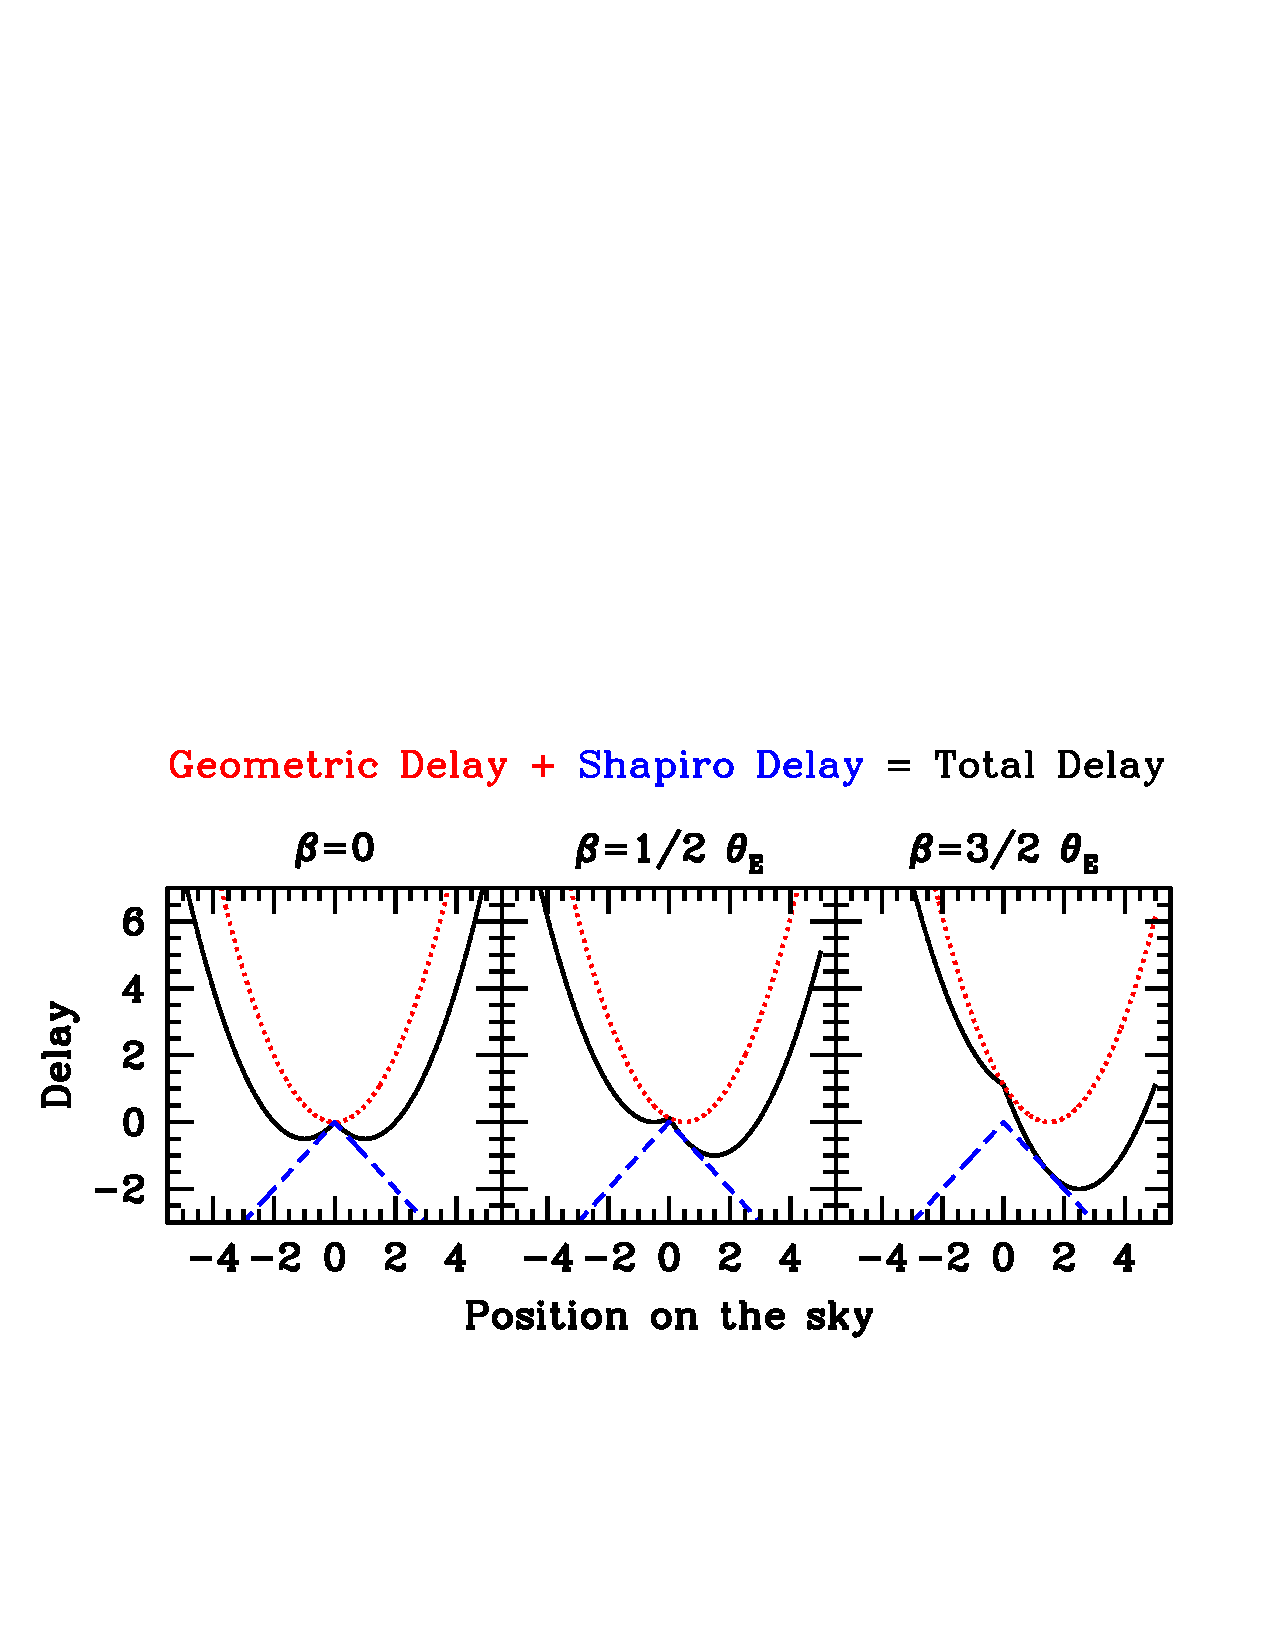
\includegraphics[width=0.96\textwidth]{figures/delays.pdf}
\caption{Geometric and general relativistic (Shapiro) contributions
to the lens time delay, from \citep{T+E15}. Images form
at minima and saddle points of the delay surface, shown here in
cross-section. Different source positions result in different
geometrical delays as well as shifted image positions.}
\label{fig:delays}
\end{figure*}

% Time delay distance.

We see from Equation~\ref{eq:timedelay} that given a mass
model that predicts $\Delta \Phi_{\rm AB}$, we can infer the ``time
delay distance'' $\Ddt$ from a measured time delay $\Delta \tau_{\rm AB}^{\rm obs}$.
This distance is actually a combination of angular diameter
distances:\footnote{As \citet{SKW06} point out, $\Ddt$ can be written more simply in terms
of comoving angular diameter distances, but most of the literature uses the
formula in Equation~\ref{eq:ddt}.}
%
\begin{equation}
    \Ddt = (1+\zd) \frac{\Dd \Ds}{\Dds}  \label{eq:ddt}
\end{equation}
%
These angular diameter distances can be predicted given the redshifts
of the lens and source, $\zd$ and $\zs$, and an assumed world model with
cosmological parameters~$\cospars$. The time delay distance is primarily
sensitive to the Hubble constant, since $\Ddt \propto H_0^{-1}$.

% Importance of mass distribution in lens.

Knowledge of the lens mass distribution is of vital importance to the
success of this cosmological inference: Equation~\ref{eq:timedelay}
shows  that the time delay  distance is as sensitive to uncertainty in
the predicted Fermat potential as it is the measured time delay itself.
More concentrated mass distributions with steeper density
profiles produce longer time delays leading to shorter inferred time
delay distances, and thus larger inferred values of $H_0$ \citep{Wuc02,Koc02,Suy12}.
% Sensitivity analysis in \citep{SKW06}? Could extend to more general
% consideration of Fermat potential difference.

% Model (mass-sheet) degeneracy and its generalizations

Moreover, there is significant risk of systematic error when modeling
lens mass distributions. While image positions remain invariant under
the ``mass sheet transformation'' \citep{FGS85,S+S13}
\citep[and its generalization, the source-position transformation][]{SPT}, the time delays
predicted by the model can change significantly. The mass sheet transformation
and its effect on the time delay is as follows:
%
\begin{align}
    \kappa(\x) \rightarrow \kappa(\x)' &= (1 - \lambda) + \lambda \kappa(\x)  \label{eq:mst} \\
    \Delta \tau \rightarrow \Delta \tau' &= \lambda \Delta \tau.
\end{align}
%
This means that if we allow our model the freedom to generate both the
$\kappa(\x)$ and $\kappa(\x)'$ mass distributions, our image position
data will not favor one over the other: they will be equally likely
given the data. This model degeneracy can only be broken by additional
information. One source of information would be independent
measurements of the mass distribution: stellar kinematics is the
obvious choice \citep{Koo++03}; sources at multiple redshifts help,
but they are rare \citep{Gav++08,Son++12} and thus not applicable in
general.

\citet{JeeKomatsuSuyu2015} provide a derivation of the resulting
cosmological dependence of kinematics-constrained power-law lens
galaxy mass models with isotropic orbits, showing that were its
density profile and velocity isotropy to be known exactly, a time
delay lens would provide a measurement of the angular diameter
distance to the lens, $\Dd$, rather than the time delay distance of
Equation~\ref{eq:ddt}. The reason given is that the velocity
dispersion and the time delay are both proportional to the enclosed
mass of the lens, but depend differently on galactocentric radius:
combining the measured velocity dispersion and time delay gives a
characteristic physical scale of the lens galaxy.  The image
separation provides a corresponding angular scale, allowing the
angular diameter distance to be probed \citep[see earlier work
by][]{GLB08}.  

In practice, the same mass model must be used to predict all of the
measured velocity dispersion, Einstein ring appearance, and time
delay, self-consistently. In the limit of low precision in the
velocity dispersion, the profile slope is weakly constrained by the
ring image alone, and the combination of time delay and lens mass
model provides information on $\Ddt$ but none on $\Dd$. As the
velocity dispersion precision increases, we expect the profile slope
to be pinned down, and the angular diameter distance to be constrained
{\it as well}. In the context of a cosmological model, the two
distances are not independent: the angular diameter distance
information provided by the velocity dispersion measurement should
translate into higher precision inference of the cosmological
parameters \citep{JeeEtal2016}.  We return to this in
Section~\ref{ssec:precision} below.

Another way to break degeneracy in the lens model is to include prior
knowledge of the lens mass distribution, from measurements of other,
similar galaxies to the lens, or perhaps from numerical
simmulations. This type of information is typically encoded as a
simply-parametrized model, such as an elliptically-symmetric mass
distribution with power law density profile (as opposed to a free form
density map; see discussion in Section~\ref{ssec:lensmodel}). Assuming
a specific density profile partially breaks the mass sheet degeneracy:
it remains to be seen hohow much systematic error in the time delay
that assumption introduces.

% Importance of mass along the line sight - the universe is not Friedmann Lemaitre Robertson Walker.

The form of the mass sheet transformation given by
Equation~\ref{eq:mst} is a rescaling plus an offset. One way to
achieve such a transformation is therefore to change the overall mass
of the lens (by a factor of $\lambda$), and at the same time add a
``mass sheet,'' a constant convergence~$(1-\lambda)$.  Both these
variations are possible in nature: lens galaxies come in a range of
masses, and the combined gravitational lensing effect of all the other
galaxies, groups and filaments along the line of sight to the source
can, in the weak lensing limit, be approximated by a constant
``external convergence'' (associate with an ``external shear'',
capable of further distorting the lensed images). However, these
physical effects only complicate the modeling problem, as one is not
allowed to assume that the mass density profile of the deflector
should vanish exactly at large radii.  The physical effect should not
be confused with the mathematical degeneracy between lens model
parameters that is associated with the mass sheet transformation, and
which would be present regardless of any external weak lensing
effects. Having said that, any additional external physical mass
component must also be taken into account when modeling the lens.

Any independent information about  the physical mass of the deflector
galaxy, such as the kinematics of its stars, can play an important role
in breaking the degeneracy in the mass model, which must now be able to
self-consistently predict the lensing effect (image distortions and time
delays) and the internal dynamics of the lens galaxy, and take into
account the weak lensing effects of structures along the line of sight.
\citet{S+S13} provide demonstrations of the scale of this problem: very
good data (both imaging and spectroscopic), as well as physically
meaningful assumptions and careful treatment of the models used, will
be needed to obtain accurate results.  In Section~\ref{ssec:lensmodel}
we review the recent choices and approximations that have been made
when constructing such models.


% \begin{figure*}
% % \centering\includegraphics[width=0.96\textwidth]{figures/line-of-sight-cartoon.pdf}
% \caption{Cartoon illustration of line of sight effects in time delay
% lens cosmography. Structures both within and outside the main lens
% plane provide weak deflections to the light rays, affecting both the
% image positions and time delays.} \label{fig:lineofsightcartoon}
% \end{figure*}


%%%%%%%%%%%%%%%%%%%%%%%%%%%%%%%%%%%%%%%%%%%%%%%%%%%%%%%%%%%%%%%%%%%%%%%%

\section{Modern time delay distance measurement [PJM]}
\label{sec:measurement}

Since 2010, it has been recognized that accurate cosmography with
individual lens systems involves the following key analysis steps.

\begin{description}
    \item{\bf Time delay estimation} The light curve extracted from
    monitoring observations is used as input to an inference of the
    time delay between the multiple images.
    \item{\bf Lens galaxy mass modeling} High resolution imaging
    and spectroscopic data are used to
    constrain a model for the lens galaxy mass distribution, which can be used
    to predict Fermat potential differences. Both the Einstein ring
    image and the stellar velocity dispersion are important.
    \item{\bf Environment and line of sight modeling} Additional observational
    information about the field of view around the lens system is used
    to account for the weak lensing effects due to massive structures in
    the lens plane and along the line of sight.
\end{description}

Cosmological parameter inference can then proceed -- although in
practice the  separation between this final step and the ones above is
not clean. Practitioners aspire to a joint inference of lens, source,
environment and cosmological parameters from all the data
simultaneously, but have to date broken the problem down  into the above
steps. In the next three sections we describe current state of the art,
limitations, and principal sources of systematic error of these three
key measurement parts of the problem.


% % % % % % % % % % % % % % % % % % % % % % % % % % % % % % % % % % % %

\subsection{Measuring time delays [PJM]}
\label{sec:measurement:timedelay}

The measurement of gravitational time delays involves two steps:  taking
monitoring observations of the system over a period of several years,
and then inferring the time delays between the multiple images from
these data.

%   %   %   %   %   %   %   %   %   %   %   %   %   %   %   %   %   %

\subsubsection{Monitoring observations and results}

Active Galactic Nuclei (AGN) show intrinsic time variability on many
scales, with the variability amplitude increasing with timescale. Long
monitoring campaigns can build up high statistical significance as
more and more light curve features can be brought into play.  However,
such long campaigns are difficult to carry out in practice, because a
large number of guaranteed observing nights are required (even if the
total exposure time is modest). Scheduling such a program has proved
difficult in traditional time allocation schemes, due to the competing
demands of the rest of the astronomy community and the long duration
requirements of lens monitoring. The highest precision time delays
have come from monitoring campaigns carried out with dedicated
facilities so far, i.e. observatories that were either able to commit
to the long term monitoring proposal submitted, or that were actually
operated in part by the monitoring collaboration.


Monitoring of the CLASS lens B1608$+$656 in the radio with the Very
Large Array enabled the breakthrough  time delay measurements of
\citep{Fas++02}. In its first season, this program  yielded measurements
of all three time delays in this quadruple image system with precision
of 6--10\% \citep{Fas++99}; with the variability of the source
increasing over the subsequent two seasons, \citep{Fas++02} were able
to reduce this uncertainty to 2--5\%. Such high precision was the
result of a dedicated campaign which consisted of 8-month seasons,
with a mean observation spacing of around 3 days. The light curves
were calibrated to 0.6\% accuracy.

While time delays had previously been measured in ten other lens
systems, this was the first time that all the delays in a quad had
been obtained; moreover, it brought the time delay uncertainty below
the systematic uncertainty due to the lens model, prompting new
efforts in this direction beyond what \citet{K+F99} needed to do.

While B1608$+$656 is not the only radio lens with measured time
delays, a combination of factors led the observational focus to shift
towards monitoring in the optical. With the sample of known, bright
lensed quasars increasing in size, networks of 1-2m class optical
telescopes began to be investigated. The variability in these systems
is somewhat more reliable, and while microlensing and image resolution
present observational challenges, the access to data was found to be
less restrictive. The COSMOGRAIL project \citep{Cou++05} took on the
task of measuring lens time delays with few-percent precision in this
way:
\citet{Eig++05} showed that microlensing was likely not to be an
insurmountable task, and \citet{Vui++07} provided the proof of concept
with a 4\% precision time delay measurement in SDSS\ J1650$+$4251.

One of the keys to the success of this program has been the simultaneous
deconvolution of the individual frames in the imaging dataset, using  a
mixture model to describe the point-like quasar images and extended lens
and AGN host galaxies \citep{MCS98}.  Another is the dedicated nature of
the network of telescopes employed, and the  careful calibration of the
photometry across this distributed system. Seasons of 8--12 months
duration over campaigns of up to 9 years have been achieved, with
typical mean observation gaps of around 3--4 days.

The COSMOGRAIL team have now published high precision time delays in
WFI\,J2033$-$4723 \citep[][3.8\%]{Vui++08}, HE\,0435$-$1223
\citep[][5.6\%]{Cou++11}, SDSS\,J1206$+$4332 \citep[][2.7\%]{Eul++13}
and  RX\,J1131$-$1231 \citep[][1.5\%]{Tew++13}, and SDSS\,J1001$+$5027
\citep[][2.8\%]{RK++13}, with more due to follow.  Typically multiple
years of monitoring is needed to obtain an accurate  time delay, as the
variability fluctuates and the reliability of the  measurement converges
\citep[see the discussion in e.g.\ ][]{Tew++13}. High precision optical time delays are also being obtained by other groups \citep{Poi++07a,Foh++07,Dah++15} using similar strategies on different telescopes.

A consistent picture seems to emerge from modern monitoring projects:
high precision gravitational time delay measurement requires campaigns
consisting of multiple, long seasons, with around 3-day cadence. The
baseline observing strategy for the Large Synoptic Survey Telescope
(LSST) is somewhat different to this, with seasons expected to be
around 4--5 months in length, and gaps between observation nights only
reaching 4--5 days when images in all filters are taken into
account. The ``Time Delay Challenge'' project was designed to test the
measurability of lens time delays with such light curves
\citep{DoblerEtal2015}, in a blind test offered to the astronomical
community. From the ten algorithms entered by seven teams, it was
concluded that time delay estimates of the precision and accuracy
needed for time delay cosmography would indeed be possible, in
$\sim$400 LSST lensed quasar systems \citep{LiaoEtal2015}. This result
came with two caveats: 1) the single filter light curve data presented
in the challenge is representative of the multi-filter data we
actually expect, and 2) that ``outliers'' (catastrophic time delay
mis-estimates) will be able to be caught during the measurement
process.  A second challenge to test these assumptions is in
preparation.



%   %   %   %   %   %   %   %   %   %   %   %   %   %   %   %   %   %

\subsubsection{Lightcurve analysis methods}

How were the time delays surveyed in the previous section derived from
the light curve data? Interest in this particular inference problem
has been high since the controversies of the late
1990's. \citet{Fas++99} used the ``dispersion method'' of
\citet{Pelt++96}, a technique that involves shifting one observed
light curve relative to another (both in time and in amplitude) and
minimizing the dispersion between adjacent points in the resulting
composite curve. Uncertainties were estimated by Monte Carlo
resampling of the data, assuming the minimum dispersion time delay and
magnification ratio to be true. In order to take into account the
slowly varying incoherent microlensing signals present in their
optical light curve data, the COSMOGRAIL team have investigated three
analysis techniques that all involve interpolation of the light curves
in some way \citep{TCM13}: free-knot splines, Gaussian processes and
simple linear interpolation have all been tested, within a common
``python curve-shifting'' (PyCS) framework.\footnote{The COSMOGRAIL
curve shifting analysis code is available from
\texttt{http://cosmograil.org}} These agree with each other given
light curves of sufficient length, providing an argument for
multiple-season monitoring campaigns.

The time delay challenge prompted seven analysis teams to develop and
test algorithms for time delay estimation. These are outlined in the
TDC1 analysis paper of \citet{LiaoEtal2015}, but we give a very brief
summary here as well, along with updated references. The PyCS team tried
a three-step approach (visual inspection and interactive curve shifting,
followed by spline fitting, followed  by an additional spline model
regression analysis of the residuals), and submitted an entry after each
step \citep{BonvinEtal2016}. Two other teams applied similar
curve-shifting approaches: both \citet{A+S2015} and \citet{RK++2015}
devised smoothing and cross-correlation schemes that they find to be
both fast and reliable. Jackson applied the dispersion method of
\citet{Pelt++96}, but carefully supervised via visual inspection to
check for  catastrophic failures.  The three remaining teams used
Gaussian Processes (GPs) to model the light curves. \citet{TakEtal2016}
used a custom Gibbs sampler to infer the hyper-parameters describing the
GP for the AGN variability and polynomials for the microlensing signals,
although they ignored microlensing during the challenge itself.
Romero-Wolf \& Moustakas implemented a very similar model, also ignored
microlensing, and used a freely-available ensemble sampler for the
inference. \citet{H+L2014} used GPs for both the AGN and microlensing
variability, and optimized the hyper-parameters rather than sampling
them.

Two factors were important in the minimisation of catastrophic time
delay mis-estimation: explicitly including microlensing in the model,
and  visual inspection of the results. An additional promising avenue
for future challenges ought to be ensemble analysis, to exploit 1) the
intrinsic correlations between, for example, AGN variability, color and
brightness, and 2) the fact that  the cosmological parameters are common
to all lens systems.


% % % % % % % % % % % % % % % % % % % % % % % % % % % % % % % % % % % %

\subsection{Modeling the lens mass distribution [TT]}
\label{sec:measurement:lensmodel}

%Preamble.

%   %   %   %   %   %   %   %   %   %   %   %   %   %   %   %   %   %

\subsubsection{High Resolution Imaging Observations}

%State of the art: HST, Keck AO.

%Limitations: resolution, bright quasar images.

%   %   %   %   %   %   %   %   %   %   %   %   %   %   %   %   %   %

\subsubsection{Lens Modeling Techniques}

%State of the art: pixelated source reconstruction,
%simply-parameterised lens mass distributions, MCMC.

%Limitations: skilled labor.

%Systematic errors: source pixelation/regularisation, lens model
%assumptions.

%   %   %   %   %   %   %   %   %   %   %   %   %   %   %   %   %   %

\subsubsection{The Role of Stellar kinematics}

% % % % % % % % % % % % % % % % % % % % % % % % % % % % % % % % % % % %

\subsection{Lens environments and line of sight effects [PJM]}
\label{sec:measurement:los}

%State of the art: ray-traced cosmological simulations, matched via
%number counts.

%Limitations/systematics: incomplete model: local vs line of sight
%mass,  ignoring multi-plane lensing, external convergence only.


%%%%%%%%%%%%%%%%%%%%%%%%%%%%%%%%%%%%%%%%%%%%%%%%%%%%%%%%%%%%%%%%%%%%%%%%

\section{From time delay distances to cosmography [PJM]}
\label{sec:cosmo}

% Approach: combining CMB and time delay distances. Blinding.

% Results. Internal consistency. Consistency with other probes.

% Combination with stellar kinematics, introduces additional
% distance dependency. Not correlated, and weaker dependence than Ddt
% (See discussion with SHS about Jee et al papers)

%%%%%%%%%%%%%%%%%%%%%%%%%%%%%%%%%%%%%%%%%%%%%%%%%%%%%%%%%%%%%%%%%%%%%%%%

\section{Outlook [TT]}
\label{sec:outlook}

%Preamble.

% % % % % % % % % % % % % % % % % % % % % % % % % % % % % % % % % %

\subsection{Precision [PJM}

FIGURE: Forecasts for 10,50,100,1000 lenses for various cosmological models (w, wa+w0, curvature etc etc). CosmoSIS forecasts (ackn. Dave \& Elise, ask them).

Check Jee et al.

%Sample size. Stage 3, stage 4 surveys. Monitoring solutions.

%Extrapolations to N lenses assuming X\% precision per time delay
%distance, forecasts.

% % % % % % % % % % % % % % % % % % % % % % % % % % % % % % % % % %

\subsection{Accuracy [PJM]}

%Addressing systematics associated with time delay measurement, lens
%modeling, environment characterisation.

%Accuracy in joint analysis: hierarchical inference.

Discussion of systematic uncertainties

Time delay measurement. Light curve quality.

Lens mass modeling. Percent-level systematics due to model assumptions (ie MSD). IFU observations, resolved stellar kinematics. Ensembles.

Environment and line of sight

Time delay perturbations (someone's noise is somebody else's signal..)

The importance of blinding.

% % % % % % % % % % % % % % % % % % % % % % % % % % % % % % % % % % % %

\subsection{Cosmic complementarity [TT]}

What's the point? Arent' other probes already doing it? Our place in the cosmology ecosystem. Discuss place relative to other distance indicators like Cepheids, BAO, Sne. Then complementarity with growth of structure probes like weak lensing, clusters etc etc. How important is H0?

Importance of multiple INDEPENDENT measurements for discovery of new physics.

%%%%%%%%%%%%%%%%%%%%%%%%%%%%%%%%%%%%%%%%%%%%%%%%%%%%%%%%%%%%%%%%%%%%%%%%

\section{Summary [TT]}
\label{sec:summary}

%%%%%%%%%%%%%%%%%%%%%%%%%%%%%%%%%%%%%%%%%%%%%%%%%%%%%%%%%%%%%%%%%%%%%%%%

%\paragraph{Paragraph headings} Use paragraph headings as needed.
%\begin{equation}
%a^2+b^2=c^2
%\end{equation}

% For one-column wide figures use
%\begin{figure}
% Use the relevant command to insert your figure file.
% For example, with the graphicx package use
%  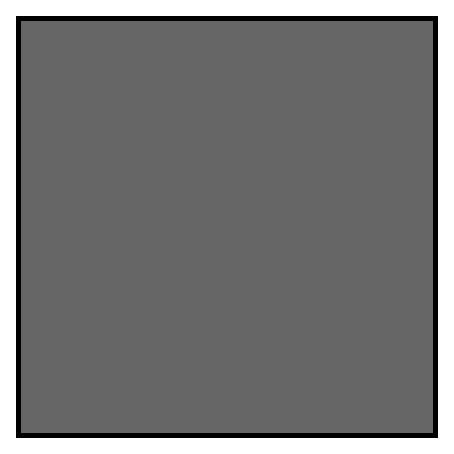
\includegraphics{example.eps}
% figure caption is below the figure
%\caption{Please write your figure caption here}
%\label{fig:1}       % Give a unique label
%\end{figure}
%
% For two-column wide figures use
%\begin{figure*}
% Use the relevant command to insert your figure file.
% For example, with the graphicx package use
%  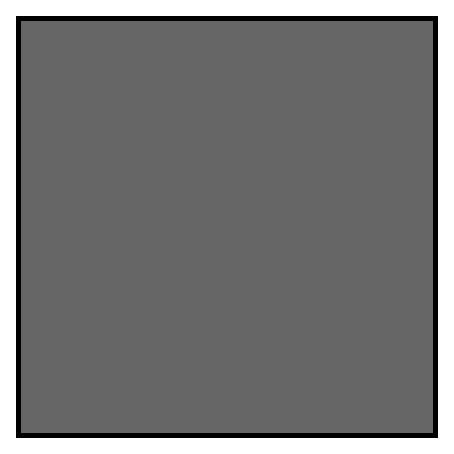
\includegraphics[width=0.75\textwidth]{example.eps}
% figure caption is below the figure
%\caption{Please write your figure caption here}
%\label{fig:2}       % Give a unique label
%\end{figure*}
%
% For tables use
%\begin{table}
% table caption is above the table
%\caption{Please write your table caption here}
%\label{tab:1}       % Give a unique label
% For LaTeX tables use
%\begin{tabular}{lll}
%\hline\noalign{\smallskip}
%first & second & third  \\
%\noalign{\smallskip}\hline\noalign{\smallskip}
%number & number & number \\
%number & number & number \\
%\noalign{\smallskip}\hline
%\end{tabular}
%\end{table}

%%%%%%%%%%%%%%%%%%%%%%%%%%%%%%%%%%%%%%%%%%%%%%%%%%%%%%%%%%%%%%%%%%%%%%%%

\begin{acknowledgements}
T.T. thanks the Packard Foundation for generous support through a
Packard Research Fellowship, the NSF for funding through NSF grant
AST-1450141, ``Collaborative Research: Accurate cosmology with strong
gravitational lens time delays''.
P.J.M. acknowledges support from the U.S.
Department of Energy under contract number DE-AC02-76SF00515.
%
Thank people who give comments/input.
\end{acknowledgements}

%%%%%%%%%%%%%%%%%%%%%%%%%%%%%%%%%%%%%%%%%%%%%%%%%%%%%%%%%%%%%%%%%%%%%%%%

% BibTeX users please use one of
\bibliographystyle{spbasic}      % basic style, author-year citations
% \bibliographystyle{spmpsci}      % mathematics and physical sciences
% \bibliographystyle{spphys}       % APS-like style for physics
\bibliography{references}   % name your BibTeX data base

% Non-BibTeX users please use
%\begin{thebibliography}{}
%
% and use \bibitem to create references. Consult the Instructions
% for authors for reference list style.
%
%\bibitem{RefJ}
% Format for Journal Reference
%Author, Article title, Journal, Volume, page numbers (year)
% Format for books
%\bibitem{RefB}
%Author, Book title, page numbers. Publisher, place (year)
% etc
%\end{thebibliography}

%%%%%%%%%%%%%%%%%%%%%%%%%%%%%%%%%%%%%%%%%%%%%%%%%%%%%%%%%%%%%%%%%%%%%%%%

\end{document}

%%%%%%%%%%%%%%%%%%%%%%%%%%%%%%%%%%%%%%%%%%%%%%%%%%%%%%%%%%%%%%%%%%%%%%%%
